\documentclass[11.5pt, onecolumn, a4paper]{article}
\usepackage[a4paper, margin=1in]{geometry}
\usepackage{graphicx}       
\usepackage[hidelinks]{hyperref} 
\usepackage{epsfig, subfigure, amsthm, amsmath} 
\usepackage{color, xcolor}  
\usepackage{setspace}       
\usepackage{tikz}           
\usepackage{enumitem}       
\usepackage{pifont}          
\usepackage[extrafootnotefeatures]{xepersian} 
\settextfont[Scale=1.2]{BZAR.TTF} 
\setlatintextfont[Scale=1]{Times New Roman} 
\usepackage[bottom]{footmisc} 

\makeatother
\setlength{\footnotesep}{1em} 
\setlength{\parindent}{1.5em} % فرورفتگی ابتدای پاراگراف
\setlength{\parskip}{0em}    % حذف فاصله بین پاراگراف‌ها
\setlength{\baselineskip}{1.5em} % فاصله بین خطوط
\setlist[itemize]{label=\ding{108}, leftmargin=2em, itemsep=0.75em} 
\renewenvironment{abstract}{%
	\noindent\textbf{\large چکیده}\\[0.5em]%
	\noindent\ignorespaces%
}{%
	\par\noindent%
}


\begin{document}
	
	\title{بهینه‌سازی خوشه‌بندی و مسیر‌یابی در شبکه‌های حسگر بی‌سیم با مدل‌های \lr{IMD-EACBR}، \lr{EECHS-ISSADE} و \lr{ABC-ACO}} 
	\author{فائزه قیاسی ، رانیا کارگر و ملیکا ملکی\\
		دانشجویان‌کارشناسی دانشگاه صنعتی اصفهان\\
		مهندسی کامپیوتر}
	\date{}
	\maketitle
	\thispagestyle{empty}
	\vfill
\section*{چکیده}
شبکه‌های حسگر بی‌سیم و اینترنت اشیا به دلیل کاربردهای گسترده در زمینه‌هایی مانند نظارت محیطی، حمل‌ونقل هوشمند و مراقبت‌های بهداشتی، اهمیت زیادی پیدا کرده‌اند. یکی از چالش‌های اصلی این شبکه‌ها، محدودیت انرژی گره‌های حسگر است که بر طول عمر شبکه تأثیر می‌گذارد. برای حل این مشکل، استفاده از تکنیک‌های مسیریابی مبتنی بر خوشه‌بندی همراه با الگوریتم‌های فراابتکاری برای انتخاب سرخوشه‌ها و طراحی مسیرهای بهینه داده‌ها پیشنهاد شده است. در این مقاله، سه مدل به‌منظور بهینه‌سازی مصرف انرژی و بهبود عملکرد شبکه ارائه می‌شوند. مدل \lr{IMD-EACBR} که از الگوریتم ارشمیدس بهبودیافته برای انتخاب سرخوشه‌ها و از الگوریتم بهینه‌سازی مبتنی‌بر آموزش و یادگیری اصلاح‌شده برای مسیریابی چندپرشی استفاده می‌کند، مدل \lr{EECHS-ISSADE} که ترکیبی از الگوریتم‌های جست‌وجوی گنجشک و تکامل تفاضلی را برای خوشه‌بندی و مسیریابی پیشنهاد می‌دهد و مدل \lr{ABC-ACO} که از الگوریتم زنبورعسل مصنوعی و کلونی مورچه‌ها برای کاهش تأخیر و توازن مصرف انرژی بهره می‌برد. نتایج شبیه‌سازی نشان می‌دهد که مدل‌های پیشنهادی در مقایسه با روش‌های قبلی، طول عمر شبکه را افزایش داده، مصرف انرژی را کاهش می‌دهند و نرخ انتقال داده‌ها را بهبود می‌بخشند. این تحقیق گامی مؤثر در بهینه‌سازی شبکه‌های حسگر بی‌سیم و اینترنت اشیا است.

	\clearpage
	\newpage
\section{مقدمه}
در سال‌های اخیر، اینترنت اشیا\LTRfootnote{Internet Of Things} و شبکه‌های حسگر بی‌سیم\LTRfootnote{Wireless Sensor Networks} به عنوان دو فناوری نوین و کلیدی، نقش مهمی در زمینه‌های مختلفی از جمله نظارت بر محیط، مراقبت‌های بهداشتی هوشمند، حمل‌ونقل هوشمند و اتوماسیون صنعتی ایفا کرده‌اند \cite{ref1, ref2, ref3}. در این شبکه‌ها، گره‌های حسگر\LTRfootnote{Sensor Nodes} به‌صورت گسترده در مناطق جغرافیایی پراکنده می‌شوند. این گره‌ها اطلاعات محیطی را جمع‌آوری کرده و به ایستگاه پایه\LTRfootnote{Base Station} ارسال می‌کنند که در شکل \ref{fig:your_label} نمونه‌ای از آن را مشاهده می‌کنید. یکی از چالش‌های اصلی این شبکه‌ها، محدودیت انرژی گره‌های حسگر است، زیرا این گره‌ها معمولاً وابسته به باتری‌های محدود هستند. مصرف سریع انرژی در گره‌ها می‌تواند باعث کاهش طول عمر شبکه\LTRfootnote{Network Lifetime} و اختلال در انتقال داده‌ها شود. به همین دلیل، بهینه‌سازی مصرف انرژی و طراحی راهکارهایی برای افزایش طول عمر شبکه از مهم‌ترین اولویت‌ها در این حوزه به شمار می‌روند.

\begin{figure}[h]
	\centering
	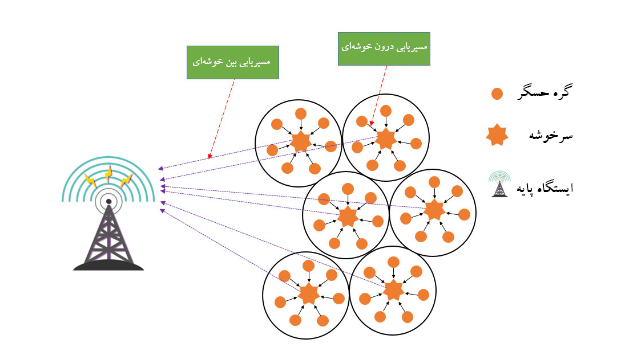
\includegraphics[width=\textwidth]{cluster-persian.png}
	\caption{یک شبکه حسگر بی‌سیم خوشه‌ای}
	\label{fig:your_label}
\end{figure}

یکی از راهکارهای مؤثر برای مقابله با محدودیت‌های انرژی در شبکه‌های حسگر بی‌سیم، استفاده از تکنیک‌های مسیریابی مبتنی بر خوشه‌بندی است. در این روش، شبکه به چندین خوشه تقسیم می‌شود و برای هر خوشه یک سرخوشه\LTRfootnote{Cluster Head} تعیین می‌گردد. سرخوشه‌ها مسئول جمع‌آوری داده‌ها از گره‌های عضو خوشه و انتقال آن‌ها به ایستگاه پایه هستند. انتخاب بهینه سرخوشه‌ها و مسیریابی داده‌ها\LTRfootnote{Data Routing} به منظور کاهش مصرف انرژی، افزایش طول عمر شبکه و بهبود کارایی، به‌ویژه در شبکه‌های بزرگ و پیچیده، اهمیت زیادی دارد.

برای انتخاب بهینه سرخوشه‌ها، الگوریتم‌های فراابتکاری\LTRfootnote{Metaheuristic Algorithms} متعددی ارائه شده‌اند. این الگوریتم‌ها با استفاده از روش‌های بهینه‌سازی پیشرفته و تحلیل پارامترهای مرتبط، نقش مهمی در کاهش مصرف انرژی و افزایش طول عمر شبکه ایفا می‌کنند. برخی از الگوریتم‌های مؤثر در این زمینه عبارتند از:

\begin{itemize}
	\item \textbf{الگوریتم بهینه‌سازی ارشمیدس بهبودیافته}\LTRfootnote{Improved Archimedes Optimization Algorithm}: این الگوریتم با بهره‌گیری از یک تابع تناسب\LTRfootnote{Fitness Function} که پارامترهایی نظیر فاصله، بهره‌وری انرژی و درجه گره را در نظر می‌گیرد، سرخوشه‌های بهینه را انتخاب می‌کند.
	\item \textbf{الگوریتم جست‌وجوی گنجشک}\LTRfootnote{Sparrow Search Algorithm}: این الگوریتم از رفتار اجتماعی گنجشک‌ها در یافتن منابع غذایی الهام گرفته و با تحلیل انرژی باقی‌مانده گره‌ها و فاصله آن‌ها از ایستگاه پایه، سرخوشه‌های بهینه را تعیین می‌کند.
	\item \textbf{الگوریتم تکامل تفاضلی}\LTRfootnote{Differential Evolution}: این الگوریتم با بهره‌گیری از روش‌های بهینه‌سازی با پیچیدگی کم و پایدار، فرآیند انتخاب سرخوشه‌ها را تسهیل می‌کند.
	\item \textbf{الگوریتم زنبورعسل بهبودیافته}\LTRfootnote{Improved Artificial Bee Colony}: این الگوریتم با الهام از رفتار زنبورها در یافتن منابع غذایی، گره‌هایی با بیشترین بهره‌وری انرژی و مناسب‌ترین موقعیت مکانی را به عنوان سرخوشه انتخاب می‌کند.
\end{itemize}

علاوه بر انتخاب سرخوشه‌ها، طراحی الگوریتم‌های بهینه برای مسیریابی داده‌ها از دیگر چالش‌های اساسی در شبکه‌های حسگر بی‌سیم است. این الگوریتم‌ها با هدف کاهش مصرف انرژی، بهبود تأخیر در انتقال داده‌ها و افزایش کارایی طراحی می‌شوند. برخی از الگوریتم‌های برجسته در این زمینه شامل موارد زیر است:

\begin{itemize}
	\item \textbf{الگوریتم مسیریابی چندپرشی مبتنی بر بهینه‌سازی آموزش و یادگیری-اصلاح‌شده‌ی ترکیبی}\LTRfootnote{Teaching-learning-Based Optimization for Multi-Hop Routing}: این الگوریتم از روش‌های بهینه‌سازی مبتنی بر آموزش و یادگیری برای یافتن مسیرهای بهینه بین گره‌ها استفاده می‌کند.
	\item \textbf{الگوریتم کلونی مورچه بهبودیافته}\LTRfootnote{Improved Ant Colony Optimization}: این الگوریتم با ایجاد مسیرهای چندپرشی بهینه از سرخوشه‌ها به ایستگاه پایه، به کاهش مصرف انرژی کمک می‌کند.
\end{itemize}


در این مقاله، سه مدل پیشنهادی برای بهینه‌سازی خوشه‌بندی و مسیریابی در شبکه‌های حسگر بی‌سیم ارائه می‌دهیم. هر مدل با استفاده از الگوریتم‌های بهینه‌سازی متنوع، سرخوشه‌های بهینه را انتخاب کرده و مسیرهای بهینه برای انتقال داده‌ها را طراحی می‌کند.

\begin{itemize}
	\item \textbf{مدل \lr{IMD-EACBR}} \cite{ref4}: این مدل از الگوریتم ارشمیدس بهبودیافته برای انتخاب سرخوشه‌ها و از الگوریتم بهینه‌سازی مبتنی‌بر آموزش و یادگیری اصلاح‌شده برای مسیریابی داده‌ها استفاده می‌کند. هدف این مدل کاهش تأخیر، متوازن‌سازی مصرف انرژی و بهبود کارایی شبکه است.
	\item \textbf{مدل \lr{EECHS-ISSADE}} \cite{ref5}: این مدل از الگوریتم‌های جست‌وجوی گنجشک و تکامل تفاضلی برای انتخاب سرخوشه‌ها و مسیریابی استفاده می‌کند. هدف اصلی این مدل کاهش مصرف انرژی و افزایش طول عمر شبکه از طریق انتخاب بهینه سرخوشه‌ها است.
	\item \textbf{مدل ترکیبی \lr{ABC-ACO}} \cite{ref6}: این مدل از الگوریتم زنبورعسل بهبودیافته برای انتخاب سرخوشه‌ها و از الگوریتم کلونی مورچه‌ها برای مسیریابی بهینه داده‌ها استفاده می‌کند. مکانیزم کنترل درون‌خوشه‌ای نیز برای کاهش مصرف انرژی در گره‌های غیرفعال به این مدل اضافه شده است.
\end{itemize}

این مقاله تلاش دارد تا با طراحی و بررسی مدل‌های پیشنهادی، گام‌های مؤثری در راستای کاهش مصرف انرژی، افزایش طول عمر شبکه و بهبود عملکرد اینترنت اشیا و شبکه‌های حسگر بی‌سیم بردارد.

\newpage
\section{کارهای مرتبط}
\subsection*{\hspace*{1em}\tikz\draw[fill=black,circle] (0,0) circle (2pt); رویکردهای ترکیبی و الگوریتم‌های بهینه‌سازی}\hspace*{2em}مطالعات اخیر به بررسی تکنیک‌های پیشرفته‌ای برای مسیریابی و خوشه‌بندی بهینه در شبکه‌های حسگر بی‌سیم \lr{(WSNs)} پرداخته‌اند که هدف آن‌ها افزایش طول عمر شبکه و بهبود عملکرد است.
کویتا و همکاران یک رویکرد ترکیبی با نام \lr{SAGA-H} را معرفی کردند که شامل الگوریتم‌های بازپخت شبیه‌سازی‌شده و ژنتیک برای مسیریابی مبتنی بر خوشه است. این روش در \lr{MATLAB} پیاده‌سازی شده و نتایج آن با الگوریتم ژنتیک معاصر مقایسه شده است. سبولاکشمی و همکاران نیز پروتکلی مبتنی بر الگوریتم بهینه‌ساز بادبان ماهی\LTRfootnote{Sailfish Optimizer (SFO)} برای بهینه‌سازی انرژی ارائه کردند\cite{ref7} که انتخاب سرخوشه‌ها را بر اساس معیارهای تناسب انجام می‌دهد. همچنین، گوودا و همکاران یک روش ترکیبی مبتنی بر شبکه عصبی\LTRfootnote{Neural Network (NN)} را پیشنهاد دادند که در آن حسگرها با استفاده از خوشه‌بندی تغییر میانگین خوشه‌بندی شده و سرخوشه‌ها با الگوریتم جستجوی عقاب طاس\LTRfootnote{Bald eagle search} انتخاب می‌شوند.
در ادامه، وایاپوری و همکاران روشی به نام  \lr{CBR-ICWSN} برای مسیریابی خوشه‌ای مبتنی بر اطلاعات ارائه کردند که از بهینه‌سازی بیوه سیاه \lr{(BWO)} برای انتخاب سرخوشه و الگوریتم مصنوعی زنبورعسل مخالف \lr{(OABC)}برای تعیین مسیر استفاده می‌کند. شفیق و همکاران نیز پروتکل مسیریابی خوشه‌ای قوی \lr{(RCBRP)} را معرفی کردند که شامل تکنیک‌های ارزیابی فاصله و مصرف انرژی است.ژنگ و همکاران رویکرد \lr{SACR} را توسعه دادند که بر پایداری خوشه‌ها تمرکز دارد، در حالی که آوان و همکاران یک استراتژی مبتنی بر بهینه‌سازی گرگ خاکستری را برای صنعت دام طراحی کردند. پاندی و همکاران نیز یک استراتژی مسیریابی چندگامی مبتنی بر یادگیری تقویتی پیشنهاد دادند که مشکلات تأخیر داده و ناکارآمدی پهنای باند را حل می‌کند.
\subsection*{\hspace*{1em}\tikz\draw[fill=black,circle] (0,0) circle (2pt); پروتکل‌های خوشه‌بندی }\hspace*{2em}روش‌های مختلفی برای بهبود عملکرد شبکه‌های حسگر بی‌سیم پیشنهاد شده‌اند. پروتکل \lr{LEACH}، یکی از نخستین الگوریتم‌های خوشه‌بندی، از انتخاب تصادفی سرخوشه‌ها استفاده می‌کند، \hspace*{.2em}اما  این روش ممکن است منجر به افزایش مصرف انرژی در برخی گره‌ها شود. الگوریتم‌های متاهیوریستیک  مانند \lr{PSO} و \lr{ABC} نیز برای بهینه‌سازی انتخاب سرخوشه‌ها معرفی شده‌اند، اما مشکلاتی نظیر همگرایی زودرس و هزینه‌های محاسباتی بالا همچنان وجود دارد.\\	
\hspace*{2em}پروتکل \lr{LEACH-C}بهبود یافته، فرآیند خوشه‌بندی را براساس مکان و انرژی گره‌ها انجام می‌دهد، اما مکانیزم مسیریابی تک‌پرشی باعث مصرف سریع انرژی در گره‌های دور از ایستگاه پایه می‌شود. پروتکل \lr{GWO} از قدرت محاسباتی ایستگاه پایه برای محاسبه دقیق انرژی مصرفی شبکه استفاده کرده و از مسیریابی دوپرشی بهره می‌برد، اما محدودیت‌هایی در پیدا کردن گره واسط مناسب دارد.\\
\hspace*{2em}پروتکل \lr{FIGWO} نیز با بهبود موقعیت شکار در \lr{GWO} طراحی شده است، اما فاقد مکانیزم مسیریابی موثر است. سایر پروتکل‌ها مانند \lr{ABC-SD} و \lr{PSO} نیز تلاش دارند تا عمر شبکه را افزایش دهند، اما تعادل بار بین سرخوشه‌ها را نادیده می‌گیرند.\\ \\
\hspace*{1em}با توجه به چالش‌های موجود در مسیریابی و خوشه‌بندی در شبکه‌های حسگر بی‌سیم، ما قصد داریم یک مکانیسم جدید مسیریابی داده ارائه دهیم که نرخ مصرف انرژی کابل‌ها را بهینه کند. این استراتژی با حفظ مصرف ثابت انرژی، سرعت انتقال داده‌ها را افزایش خواهد داد. آزمایش‌ها با استفاده از شبیه‌سازی و استقرار گره‌های واقعی در یک بستر آزمایشی \lr{WSN} انجام خواهد شد. همچنین، برای جلوگیری از رفتار خودخواهانه گره‌های حسگر، یک ابزار پیامد مبتنی بر نظریه بازی طراحی خواهد شد که گره‌ها را به پذیرش روش‌های مشارکتی ترغیب می‌کند. پیش‌بینی می‌شود این روش بتواند مصرف انرژی شبکه را کاهش داده و میزان انتقال داده‌ها را افزایش دهد که منجر به بهبود طول عمر شبکه خواهد شد.\\
\section{مدل پیشنهادی}
\hspace*{2em}مدل \lr{EECHS-ISSADE} بر اساس رفتارهای طبیعی  گنجشک‌ها طراحی شده است. گنجشک‌ها از استراتژی‌های جستجوی غذا و اجتناب از شکار برای یافتن منابع استفاده می‌کنند. در این مدل، \lr{SSA} به عنوان یک ابزار جستجوی سریع عمل می‌کند و \lr{DE} به منظور جلوگیری از گرفتار شدن در بهینه‌های محلی و تقویت قابلیت جستجوی جهانی به کار می‌رود. تابع برازندگی این مدل شامل پارامترهایی نظیر انرژی باقی‌مانده، فاصله درون خوشه‌ای و فاصله سرخوشه تا ایستگاه پایه است. این پارامترها به طور پویا برای هر گره محاسبه شده و بهینه‌ترین سرخوشه‌ها انتخاب می‌شوند. \lr{SSA} برای شبیه‌سازی رفتارهای اسپارو و \lr{DE} برای بهبود فرایند جستجو و جلوگیری از همگرایی زودهنگام ترکیب شده‌اند. این مدل به طور خاص تضمین می‌کند که گره‌هایی با انرژی پایین به عنوان \lr{CH} انتخاب نشوند، در حالی که گره‌هایی با انرژی بالا به طور عادلانه بار مسئولیت را تحمل می‌کنند.\\
پروتکل پیشنهادی شامل دو بخش اصلی است:\\
\hspace*{1em}1.خوشه‌بندی: در این مرحله، گره‌های حسگر به خوشه‌هایی تقسیم شده و یک گره به عنوان سرخوشه انتخاب می‌شود. انتخاب سرخوشه‌ها با استفاده از الگوریتم \lr{IABC} انجام می‌شود که معیارهایی نظیر انرژی باقی‌مانده، تراکم گره‌ها و فاصله را در نظر می‌گیرد.\\
\hspace*{1em}2.مسیریابی: پس از تشکیل خوشه‌ها، داده‌های حسگرها به سرخوشه‌ها منتقل شده و سپس از طریق مسیرهای چندگامی\LTRfootnote{Multi-Hop Paths} به ایستگاه پایه ارسال می‌شوند. این مسیرها با استفاده از الگوریتم بهبود یافته \lr{ACO} تعیین می‌شوند تا مصرف انرژی بهینه شود.


\section{مطالعه شبیه سازی}
\hspace*{1em}برای ارزیابی عملکرد مدل \lr{EECHS-ISSADE}، شبیه‌سازی‌هایی در  \lr{MATLAB}  انجام شد. شبکه‌ای به ابعاد 200×200 متر با 100 گره حسگری همگن طراحی شد. این گره‌ها به طور تصادفی در شبکه توزیع شدند و ایستگاه پایه در مرکز شبکه قرار گرفت. مدل پیشنهادی با الگوریتم‌های \lr{LEACH}، \lr{TABU-PSO} و \lr{EECHS-ABC} مقایسه شد. پارامترهایی مانند تعداد گره‌های زنده، انرژی باقی‌مانده، نرخ انتقال داده و پایداری شبکه به عنوان معیارهای ارزیابی انتخاب شدند. نتایج نشان داد که \lr{EECHS-ISSADE} در حفظ تعداد بیشتری از گره‌های زنده برای دوره‌های طولانی‌تر موفق عمل کرده است. همچنین، مصرف انرژی در این مدل به طور قابل ملاحظه‌ای کاهش یافت و نرخ انتقال داده به ایستگاه پایه افزایش پیدا کرد.\\	

\newpage
\begin{thebibliography}{9}

	\begin{LTR}	
		{\bibitem{ref1} \lr{Sharma, Deepak, and Amol P. Bhondekar. "Traffic and energy aware routing for heterogeneous wireless sensor networks." \textit{IEEE Communications Letters} 22.8 (2018): 1608-1611.}}
		
		\bibitem{ref2} \lr{Farsi, Mohammed, et al. "A congestion-aware clustering and routing (CCR) protocol for mitigating congestion in WSN." \textit{IEEE Access} 7 (2019): 105402-105419.}
		
		\bibitem{ref3} \lr{Satpathy, Sambit, et al. "Design a FPGA, fuzzy based, insolent method for prediction of multi-diseases in rural area." \textit{Journal of Intelligent \& Fuzzy Systems} 37.5 (2019): 7039-7046.}
		
		\bibitem{ref4} \lr{Kathiroli, Panimalar, and Kanmani Selvadurai. "Energy efficient cluster head selection using improved Sparrow Search Algorithm in Wireless Sensor Networks." \textit{Journal of King Saud University-Computer and Information Sciences} 34.10 (2022): 8564-8575.}
		
		\bibitem{ref5} \lr{Lakshmanna, Kuruva, et al. "Improved metaheuristic-driven energy-aware cluster-based routing scheme for IoT-assisted wireless sensor networks." \textit{Sustainability} 14.13 (2022): 7712.}
		
		\bibitem{ref6} \lr{Wang, Zongshan, et al. "An energy efficient routing protocol based on improved artificial bee colony algorithm for wireless sensor networks." \textit{IEEE Access} 8 (2020): 133577-133596.}
		
		\bibitem{ref7} \lr{Mohan, Prakash, et al. "Improved metaheuristics-based clustering with multihop routing protocol for underwater wireless sensor networks." \textit{Sensors} 22.4 (2022): 1618.}
		
	\end{LTR}
\end{thebibliography}


\end{document}

